\documentclass[11pt]{beamer}
\usetheme{Warsaw}
\usepackage[utf8]{inputenc}
\usepackage[english]{babel}
\usepackage{amsmath}
\usepackage{amsfonts}
\usepackage{amssymb}

%expectations
\newcommand{\expect}{\mathbb{E}}

\AtBeginSection[]{
  \begin{frame}
  \vfill
  \centering
  \begin{beamercolorbox}[sep=8pt,center,shadow=true,rounded=true]{title}
    \usebeamerfont{title}\insertsectionhead\par%
  \end{beamercolorbox}
  \vfill
  \end{frame}
}


\begin{document}
%%%%%%%%%%%%%%%%%%%%%%%%%%%%%%%%%%%%%%%%%%%%%%%%%%%%%%%%
\begin{frame}
  \frametitle{}
  \begin{center}
    \textbf{\large MATH 4281 Risk Theory--Ruin and Credibility}\\
    \vspace{1cm}
    {\large  Module 2: Ruin Theory (cont.) } \\
    \vspace{1cm}
    {\large  Feb 23, 2021}
    \end{center}
    \vspace{1cm}
\end{frame}
%%%%%%%%%%%%%%%%%%%%%%%%%%%%%%%%%%%%%%%%%%%%%%%%%%%%%%%%
\begin{frame}
\tableofcontents
\end{frame}
%%%%%%%%%%%%%%%%%%%%%%%%%%%%%%%%%%%%%%%%%%%%%%%%%%%%%%
\section{Post Reading Week/test \#1 Review}
\begin{frame}{Recall the following}

Since it's been since the 4th we will review what we covered of Ruin Theory so far. Recall we covered: 

\begin{itemize}

\item Stochastic processes and their properties (independent \textbackslash stationary increments, etc...) .

\item Counting processes, specifically Poisson processes. 

\item Compound Poisson processes.

\item Leading to the \alert{Cram\'er-Lundberg process}:

$$U(t)=\underbrace{u_0+ct}_\text{Revenue} - \underbrace{\sum_{i=1}^{N(t)}X_i}_\text{\alert{Losses}}$$ 

\end{itemize}



\end{frame}
%%%%%%%%%%%%%%%%%%%%%%%%%%%%%%%%%%%%%%%%%%%%%%%%%%%%%%
\begin{frame}{The probability of ruin}

\begin{itemize}

\item Recall the Cram\'er-Lundberg model:

$$U(t)= u_0+ct - \sum_{i=1}^{N(t)}X_i$$

\item The time to ruin $T$ is defined as
$$T=\inf \{ t\ge 0 | U(t)<0\}.$$

\item The probability that the company would be ruined by time $t$ is denoted by
$$\psi(u_0,t)=\Pr[T<t].$$

\end{itemize}

\end{frame}
%%%%%%%%%%%%%%%%%%%%%%%%%%%%%%%%%%%%%%%%%%%%%%%%%%%%%%%%
\begin{frame}{Avoiding Ultimate Ruin}

\begin{itemize}

\item Finally, the probability of \alert{ultimate} ruin is
$$\psi(u_0) =\Pr(T<\infty)= \lim_{t\rightarrow \infty} \psi(u_0,t) \ge \psi(u,t).$$

\vfill

\item The Net Profit Condition (NPC):

\begin{equation*}\label{Def:NPC}
c \leq \lambda \expect[X_i] \Rightarrow \psi(u_0)=1
\end{equation*} 
\vfill
\item To ensure the NPC holds we add our "safety loading" : 

\begin{equation*}
c=(1+\theta)\lambda \expect[X]
\end{equation*}
\end{itemize}

\end{frame}
%%%%%%%%%%%%%%%%%%%%%%%%%%%%%%%%%%%%%%%%%%%%%%%%%%%%%%%
\begin{frame}{Recall we introduced an approximation}

We can approximate $\psi$ easy via \alert{The Lundberg Inequality}:
\vfill
\begin{equation*}\label{Def:LI1}
\psi(u) \leq e^{-Ru } 
\end{equation*} 
\vfill
Where R (the adjustment coefficient) solves the equation\footnote{Where $S_t=\sum_{i=1}^{N(t)} X_i$}
\begin{equation*}\label{Def:NPC}
e^{r p t} = \expect[e^{r S_t }]
\end{equation*} 
\vfill
Today we will discuss this in more detail.

\end{frame}
%%%%%%%%%%%%%%%%%%%%%%%%%%%%%%%%%%%%%%%%%%%%%%%%%%%%%%%
\section{The Lundberg Inequality}
\begin{frame}{Avoiding Ultimate Ruin}

In the Cram\'er-Lundberg model, consider the excess of losses over premiums over the interval $[0,t]$: $S(t)-ct.$ We define the \alert{adjustment coefficient $R$} as the first positive solution of the following equation in $r$:


$$M_{S(t)-ct}(r)=E\left[ e^{r(S(t)-ct)} \right]=e^{-rct}e^{\lambda t [M_X(r)-1]}=1,$$

\vfill

Recall $c = (1 + \theta) \lambda E[X]$. So, the adjustment coefficient $R$ is the first positive of the following equation:

\begin{eqnarray*}
1+(1+\theta) rE[X] = M_X(r)
\end{eqnarray*}



\end{frame}
%%%%%%%%%%%%%%%%%%%%%%%%%%%%%%%%%%%%%%%%%%%%%%%%%%%%%%
\begin{frame}{Does such an $R$ exist?}

\begin{figure}
\centering
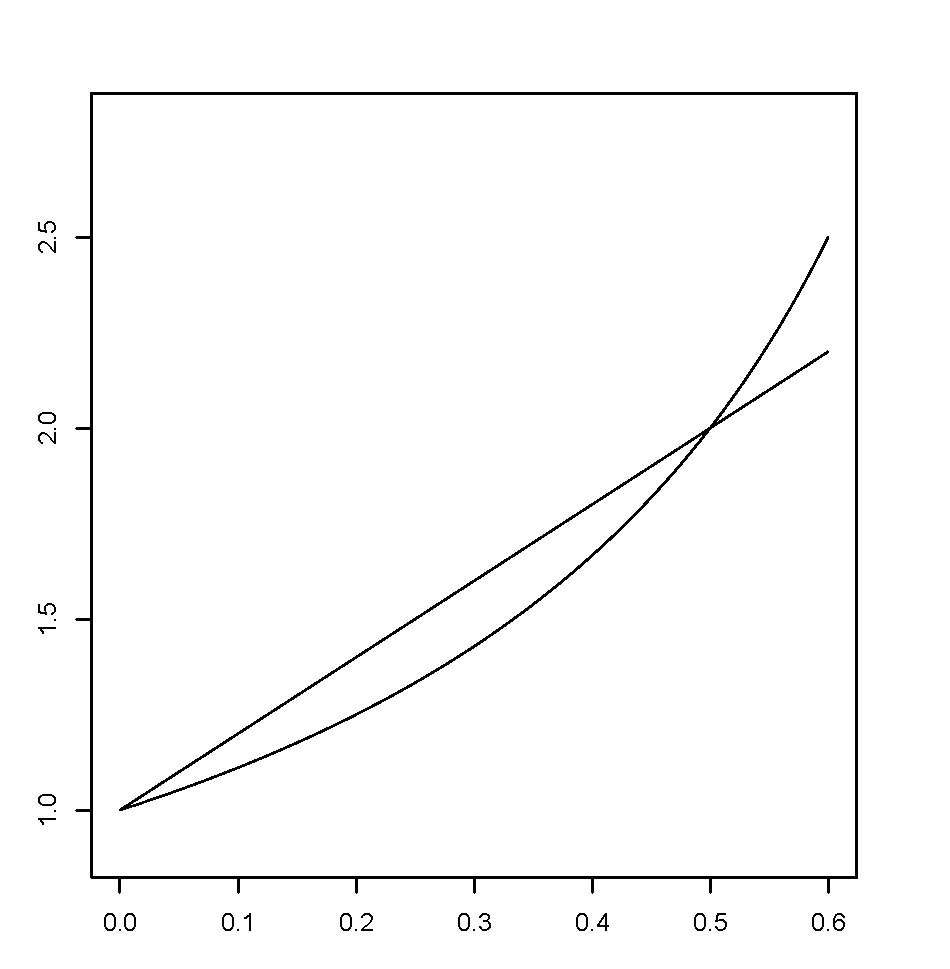
\includegraphics[scale=0.35]{Rplot}
%\caption{}
\end{figure}
{\small
\begin{itemize}
\item Recall~that~Jesen's~inequalty~gives~$1+(1+\theta) rE[X] = M_X(r) \geq e^{rE[X]}$ 

\item How else could this fail?
\end{itemize}
}



\end{frame}
%%%%%%%%%%%%%%%%%%%%%%%%%%%%%%%%%%%%%%%%%%%%%%%%%%%%%%
\begin{frame}{The Theorem}
\begin{enumerate}
\item Let $R > 0$ be the adjustment coefficient. If $\{U(t)\}$ is a Cram\'er-Lundberg process with $\theta>0$, then for $u\ge 0$
$$\psi(u)=\frac{e^{-Ru}}{E\left[ e^{-R U(T)} | T<\infty\right]}.$$
\item Since $U(T)<0$, we have then (Lundberg's exponential upper bound)
$$\psi(u)< e^{-Ru}.$$
\end{enumerate}
\end{frame}
%%%%%%%%%%%%%%%%%%%%%%%%%%%%%%%%%%%%%%%%%%%%%%%%%%%%%%
\begin{frame}{An Example} 
\vspace{- 4.5 cm}
Assume $X\sim\text{exp}(\beta)$ (the mean is $1/\beta$). Find $R$ and $\psi(u)$.

\end{frame}
%%%%%%%%%%%%%%%%%%%%%%%%%%%%%%%%%%%%%%%%%%%%%%%%%%%%%%
\begin{frame}{An Example}

\end{frame}
%%%%%%%%%%%%%%%%%%%%%%%%%%%%%%%%%%%%%%%%%%%%%%%%%%%%%%
\section{Proving the Cram\'er-Lundberg Inequality}
\begin{frame}{Proving our theorems}



\vspace{- 4.5 cm} To start show that $\left\{e^{-R U(t)}\right\}$ is a martingale\footnote{i.e. $E\left[ e^{-R U(t)}| e^{-R U(s)}\right]=e^{-RU(s)}$ for $s<t$ or $E\left[ e^{-R U(t)}\right]=e^{-Ru}$ for all $t$}



\end{frame}
%%%%%%%%%%%%%%%%%%%%%%%%%%%%%%%%%%%%%%%%%%%%%%%%%%%%%%
\begin{frame}{A \textit{very very} useful theorem}

(Given we don't have all the machinery we need at this point- we will define a \emph{stopping time} as a random time dependent on another stochastic process exhibiting some behaviour)

\begin{theorem}[Optimal Stopping Theorem]
Given a \emph{bounded} stopping time $T$, i.e. $T\leq t_0 < \infty$ for a martingale\footnote{For those who know we must also impose right continuity} $M_t$ them:

$$ M_0 = E[M_T] $$

\end{theorem}

\end{frame}
%%%%%%%%%%%%%%%%%%%%%%%%%%%%%%%%%%%%%%%%%%%%%%%%%%%%%%
\begin{frame}{An example: Gambler's Ruin}
\vspace{-3 cm}
A gambler enters a casino with $n$ dollars and plays a game with a win probability $p$. He gains \$1 for every win and losses \$1 for every loss. He leaves when he wins $N$ or looses everything. What is the probability he leaves ruined?

\end{frame}
%%%%%%%%%%%%%%%%%%%%%%%%%%%%%%%%%%%%%%%%%%%%%%%%%%%%%%
\begin{frame}{An example: Gambler's Ruin}

\end{frame}
%%%%%%%%%%%%%%%%%%%%%%%%%%%%%%%%%%%%%%%%%%%%%%%%%%%%%%
\begin{frame}{Proof of the Cram\'er-Lundberg Inequality}



\end{frame}
%%%%%%%%%%%%%%%%%%%%%%%%%%%%%%%%%%%%%%%%%%%%%%%%%%%%%%
\begin{frame}{Proof of the Cram\'er-Lundberg Inequality}

\end{frame}

\end{document}